\begin{tikzpicture}[align=center,
    node distance=0.7cm and 0.7cm,
    every initial by arrow/.style={draw=none, minimum size=0em},
    %node styles:
    block_center/.style ={rectangle, draw=black, thick, fill=white,
            text width=8em, text centered, minimum height=4em},
    block_left/.style ={rectangle, draw=black, thick, fill=white,
            text width=16em, text ragged, minimum height=4em, inner sep=6pt},
    block_noborder/.style ={rectangle, draw=none, thick, fill=none,
            text width=18em, text centered, minimum height=1em},
    block_assign/.style ={rectangle, draw=black, thick, fill=white,
            text width=18em, text ragged, minimum height=3em, inner sep=6pt},
    block_lost/.style ={rectangle, draw=black, thick, fill=white,
            text width=16em, text ragged, minimum height=3em, inner sep=6pt},
    block_rounded/.style ={rectangle, draw=black, thick, fill=white,
            text width=8em, text centered, rounded corners=.55cm, minimum height=4em},
    line/.style ={draw, very thick, line cap=round, -{Latex[length=2.5mm]}, shorten >=0pt}
    ]

    \matrix [column sep=20mm,row sep=3mm] (mtx) {
        \node[inner sep=0pt] (user) {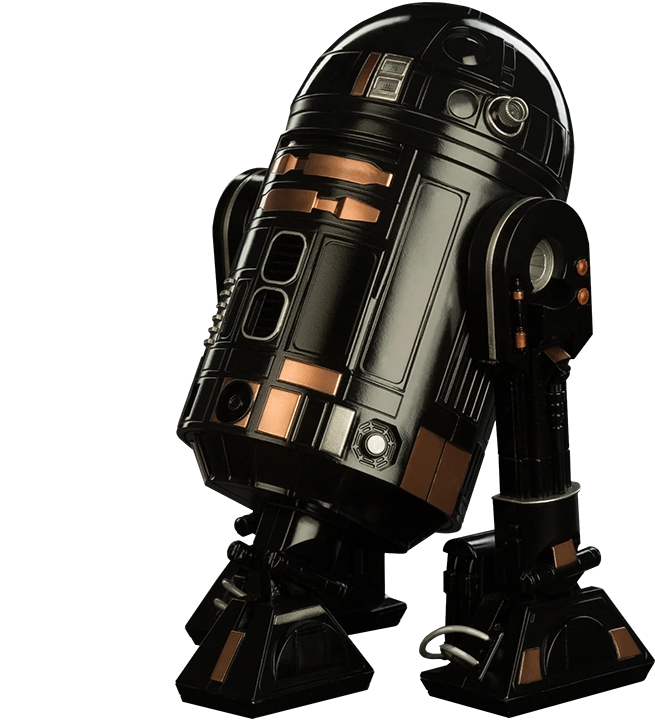
\includegraphics[height=.2\textheight]{img/astromech.png}};
         & \node [inner sep=0pt] (server) {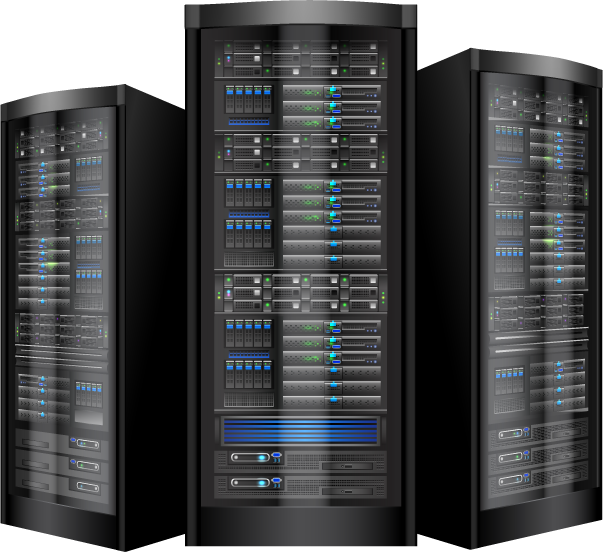
\includegraphics[height=.2\textheight]{img/server.png}}; \\
    };


    \path[draw, line]
    (user) edge [out=45, in=135] node[above] {Sensory Input} (server)
    (server) edge [out=225, in=315] node[below] {Human-parseable\\Feedback} (user);
\end{tikzpicture}